\documentclass{article}

\usepackage[margin=1in]{geometry}
\usepackage{amssymb, amssymb, amsthm}
\usepackage{enumitem}
\usepackage{courier}
\usepackage{listings}
\usepackage{graphicx}
\usepackage{fancyvrb}
\usepackage{color}
\usepackage{hyperref}
\lstset
{
    language=Python,
    numbers=left,
    stepnumber=1,
    showstringspaces=false,
    tabsize=4,
    breaklines=true,
    breakatwhitespace=false,
}

\begin{document}
\pagenumbering{gobble}

\begin{flushright}
Keegan Dahm \\
CYBER W207 \\
Lab 3
\end{flushright}

This writeup is also on GitHub at \href{https://github.com/TehVulpes/W207-Lab-3}{https://github.com/TehVulpes/W207-Lab-3}

\begin{enumerate}[start=1]
\item % 1
    The training data had 126 columns. PCA quickly caught up, and was able to explain 90\% of data variance with only 30 components, which can significantly reduce model training costs.
    
    \begin{center}
    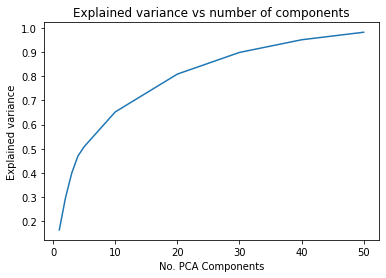
\includegraphics[width=5cm]{part1.0.png}
    \end{center}

\item % 2
    For this, I generated a second graph, where non-poisonous samples are semi-transparent. This helps show the overlap between the two categories after 2-component PCA.
    
    \begin{center}
    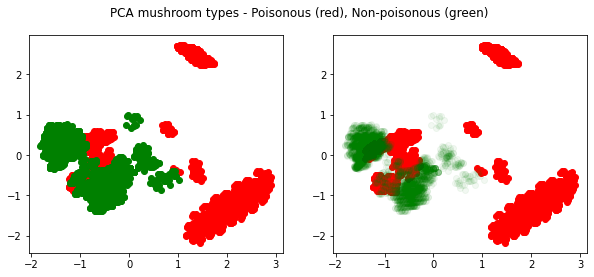
\includegraphics[width=10cm]{part2.0.png}
    \end{center}
    
    As this chart shows, some poisonous clusters end up distinctly separated from the rest and are easily distinguishable, while some clusters overlap, and would need more components to tell apart.
    
\item % 3
    After K-Means clustering, the results showed significant overlap between the clusters found. The edges of the clusters were seemingly defined by the edges where they stopped overlapping with each other.
    
    \begin{center}
    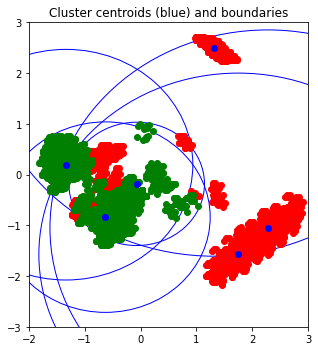
\includegraphics[width=5cm]{part3.0.png}
    \end{center}
    
\newpage

\item % 4
    As expected, increasing the number of GMM components improves the fi delity of the GM clustering. For this dataset, the full covariance type best fit the shape of the clusters.
    
    \begin{center}
    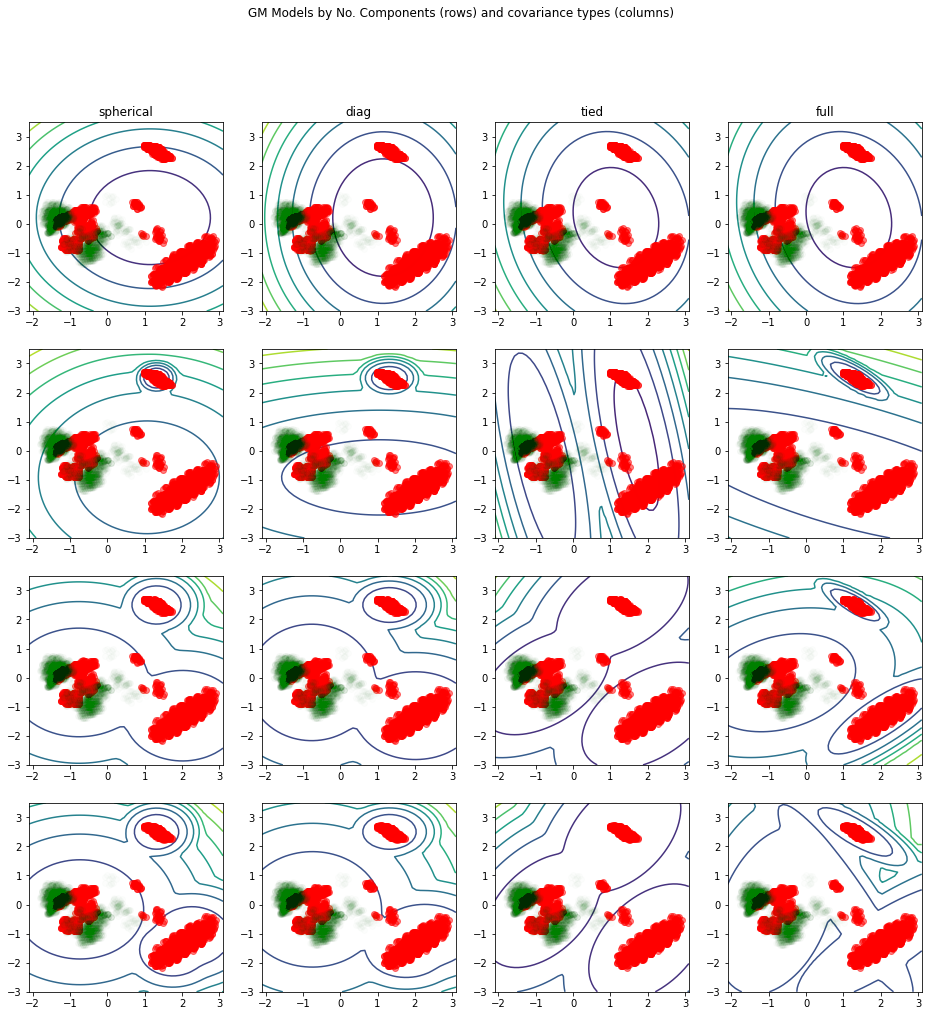
\includegraphics[width=10cm]{part4.0.png}
    \end{center}

\item % 5
    For parts 5 and 6, it looks like some of the code was already written, and looking at Google Drive, the ipynb was last modified July 21, so I'm assuming we're allowed to build off of the existing code.
    
    Running the scoring code found that, alone, the positive / negative models had very low accuracy. The positive model had about 20.1\% accuracy, while the negative model had about 19.6\% accuracy. Combined, however, they performed very well, with 95.0\% accuracy. This shows the usefulness of ensembling different models, to pick and choose each one's strengths while ignoring its weaknesses.
    
\item % 6
    Like part 5, some of the code was already written. I added code to train \texttt{gmm\_p} and \texttt{gmm\_n}, to generate predictions from each GM model, and to score them. Running this cell produced the following output:
    
    \texttt{The best GMM had 2 PCA components, 5 GMM components, full covariance type, \\and 50.0 parameters. \\
    It had an accuracy of 0.9564056939501779}
    
    This found that PCA doesn't necessarily have to explain all the variance to produce useful, reduced workspaces.
    
\end{enumerate}

\end{document}
